%!TEX TS-program = xelatex
\documentclass[]{friggeri-cv}
\usepackage{afterpage}
\usepackage{hyperref}
\usepackage{color}
\usepackage{xcolor}


\hypersetup{
    pdftitle={},
    pdfauthor={},
    pdfsubject={},
    pdfkeywords={},
    colorlinks=false,       % no lik border color
   allbordercolors=white    % white border color for all
}
\addbibresource{bibliography.bib}
\RequirePackage{xcolor}

\begin{document}
\header{ \hspace{10mm} Georgios}{\hspace{4mm}Manakanatas}{\hspace{65mm}Software Engineer\cdotp Consultant}%\hspace{40mm}Software Engineer

% Fake text to add separator      
\fcolorbox{white}{gray}{\parbox{\dimexpr\textwidth-2\fboxsep-3\fboxrule}{.....}}

% In the aside, each new line forces a line break
\begin{aside}
  \section{Address}
    Draakstraat, 32
    2018, Antwerp, Belgium
  \section{Contact info}
    
\includegraphics[width=0.4cm]{img/phone.png} +30 6977 138253
    
\includegraphics[width=0.4cm]{img/skype.png} george.manakanatas
    
\includegraphics[width=0.4cm]{img/mail.png} \hspace{0.5 mm} \href{mailto:manakanatas@gmail.com}{manakanatas@\\gmail.com}   
  \section{Web \& Git}
    
\includegraphics[width=0.4cm]{img/Linkedin.png} \hspace{0.5 mm} \href{http://www.linkedin.com/in/george-manakanatas}{www.linkedin.com /in/george-manakanatas}
    
\includegraphics[width=0.4cm]{img/github.png} \hspace{0.5 mm} \href{https://github.com/GeorgeManakanatas}{https://github.com/ GeorgeManakanatas}
    
\includegraphics[width=0.4cm]{img/web.png} \hspace{0.5 mm} \href{https://georgemanakanatas.github.io/}{https://george manakanatas.github.io/}
  \section{Programming \\ Languages}
  ~
  
\includegraphics[scale=0.45]{img/newLanguages2.png}
  \section{Human \\ Languages}
    \textbf{Dutch}
\includegraphics[scale=0.40]{img/1stars.png}
    \textbf{English}
\includegraphics[scale=0.40]{img/5stars.png}
    \textbf{German}
\includegraphics[scale=0.40]{img/3stars.png}
    \textbf{Greek}
\includegraphics[scale=0.40]{img/5stars.png}
  \section{OS Experience}
    \textbf{Linux}
\includegraphics[scale=0.40]{img/5stars.png}
    \textbf{MacOS}
\includegraphics[scale=0.40]{img/1stars.png}
    \textbf{Windows}
\includegraphics[scale=0.40]{img/4stars.png}
    ~
\end{aside}
~
\section{Experience}

\begin{entrylist}
  \entry
    {04/2016 - \\This day}
    {Software Engineer}
    {Apogado CVBA, Mechelen, Belgium}
    {Working for Apogado my time is split between back end development, software architecture, and consulting.\par
    \hspace{15pt}As a developer I focus mostly on the back end with most of my code written in Java, JavaScript and Python. I am comfortable working on and have experience with both the LAMP and MEAN stacks working both with legacy code as well as on new projects. With SOAP and REST protocols, with relational (MySQL ,MariaDB) and non relational (MongoDB) databases as well as automated testing.\par My Java projects so far lean heavily on Apache service mix components and have been mostly geared towards data transformation as well as service oriented integration for accessing and providing added value to the information of the various authentic sources of the Belgian federal state.\par My JavaScript work has been on back end development of a proprietary  Apogado GDPR compliance tool built on the MEAN stack. \par Over the last year I have also placed high emphasis on developing skills on automated testing, continuous integration as well as infrastructure as code while using Python for ad hoc scripting when needed.\par
    \hspace{15pt}As an architect I help evaluate existing or proposed architectures as well as identify security gaps and recommend fixes or enhancements. I also design and build security for products from scratch as well as their associated databases taking care to balance business and information security requirements.\par
    \hspace{15pt}As a consultant I help design and/or implement custom made solutions tailored to a specific client’s needs as part of the Apogado team.}
  \entry
    {09/2014 - \\09/2015}
    {Master's Thesis}
    {Hellenic Open University, Patra, Greece}
    {Knowledge hiding and Association rule hiding, hiding frequent itemsets, exact knowledge hiding through database extension, k-anonnymity, Rob frugal anonymisation, Apriori data mining algorithm. Python programming, tkinter GUI package, LaTeX text editor.}
  \entry
    {09/2004 - \\09/2015}
    {Physics and Mathematics tutor}
    {Freelance, Heraclion \& Athens, Greece}
    {Physics and Mathematics tutoring for high school and junior high school students. Advanced Physics and Mathematics classes for College students, preparatory courses for end of semester examinations. }
    
\end{entrylist}

\newpage

\begin{aside}
~
  \section{Tools \& \\Frameworks}
    ~
    
\includegraphics[scale=0.2]{img/newTools2.png}
    ~
  \section{Hobbies \& \\Interests }
    ~
    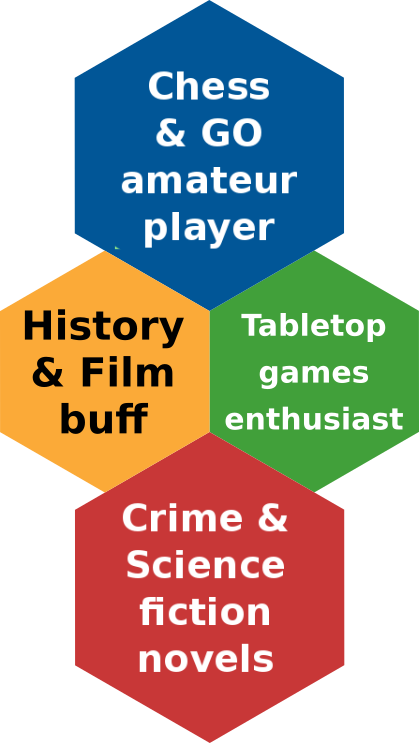
\includegraphics[scale=0.20]{img/personal.png}
    ~
 \section{Places Lived}
    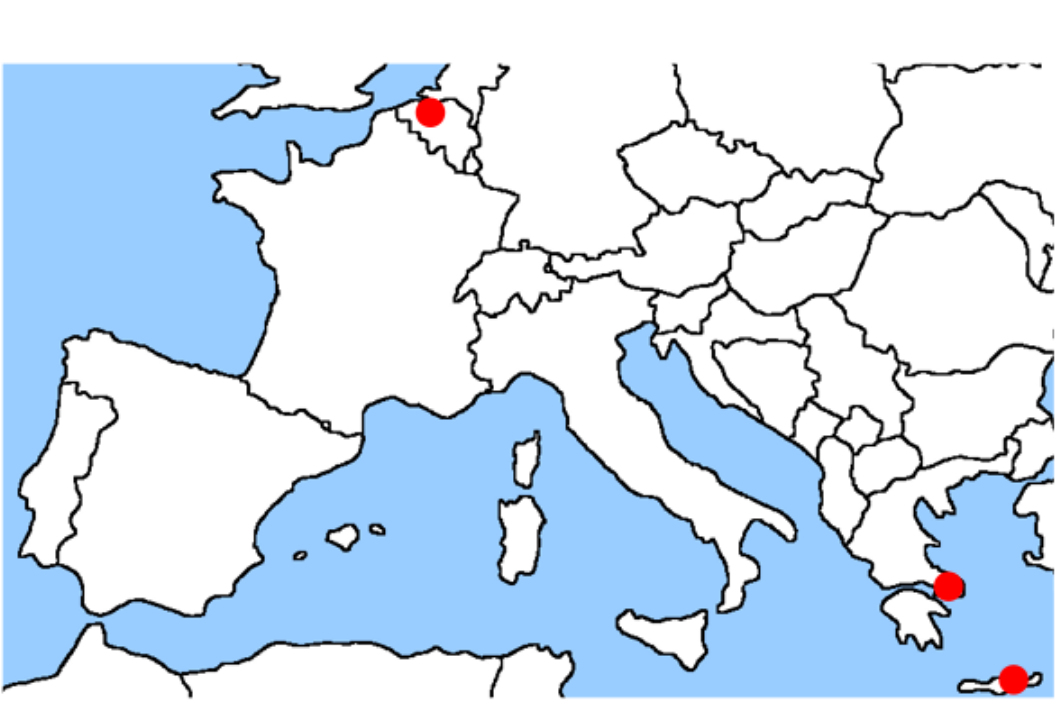
\includegraphics[scale=0.10]{img/europe_map_me.png}
    ~
\end{aside}
~
\section{Education}
\begin{entrylist}
  \entry
    {2012 - \\2015}
    {Master's Degree in Information Systems}
    {Hellenic Open University, Patra, Greece}
    {Curriculum: Information and Communication Technologies.\\
    Main subjects: Computer Networks and Communications, Computer Architecture, Software Engineering, Software Design and Management Processing.\\
    \emph{Title of the Thesis: ”Blocking Inference Channels in Outsourced Data Mining.”}\\
    \emph{Relators: Prof. Ilias Stauropoulos, Prof. Basilios Berikios.}}
  \entry
    {2000 - \\2009}
    {Bachelor's Degree in Physics}
    {University of Crete, Heraklion, Greece}
    {Curriculum: Physics and Mathematics.\\ 
    Main subjects: Classical Mechanics, Electromagnetism, Thermodynamics and Statistics, Quantum Physics, Atmospheric Physics, Introduction to Circuit theory, Applied Geophysics, Elements of Electronics, Introduction to Optoelectronics, Financial Mathematics, Computational Physics.}
\end{entrylist}
~
\section{Skills}
\textbf{Programming}\\
Good knowledge of Java, JavaScript and Python. Also XML, XSL, JSON, YAML.  \\Working Knowledge of SQL, Bash and C.\\
\textbf{Frameworks \& Databases}\\
Good knowledge of Node.js, Express.js, MongoDB, MariaDB, MySQL, Apache CXF, Apache Camel, Apache Karaf, Spring. \\Working knowledge of the Talend ESB. Basic knowledge of Django, AngularJS, bootstrap.\\
\textbf{Tools}\\
Good knowledge of Postman, SoapUI, Ansible, Docker,\\
Working knowledge of Selenium, Jenkins, OpenAPI, Apache Maven, Talend Open Studio \\
\textbf{General}\\ 
Solid mathematical background and analytic skills from my physics studies. Basic knowledge of Data mining as well as data anonymization and de-identification methods.
\\
\section{Certifications}
    \textbf{English :}
    Near Native Fluency, Certificate of Proficiency in English, University of Cambridge\\
    \textbf{German :}
    Fluent, Zeugnis Zentrale Mittelstufenprüfung, Goethe Institut\\
    \textbf{Greek :}
    Native Speaker
\\
\section{Other Info}
European driving licence, Belgian certificate of registration. For the Greek job market: Στρατιωτικές υποχρεώσεις εκπληρωμένες, φορολογικός κάτοικος εξωτερικού.
\begin{flushleft}
\emph{January, 2018}
\end{flushleft}
\begin{flushright}
\emph{Georgios Manakanatas}
\end{flushright}

%%% This piece of code has been commented by Karol Kozioł due to biblatex errors. 
% 
%\printbibsection{article}{article in peer-reviewed journal}
%\begin{refsection}
%  \nocite{*}
%  \printbibliography[sorting=chronological, type=inproceedings, title={international peer-reviewed conferences/proceedings}, notkeyword={france}, heading=subbibliography]
%\end{refsection}
%\begin{refsection}
%  \nocite{*}
%  \printbibliography[sorting=chronological, type=inproceedings, title={local peer-reviewed conferences/proceedings}, keyword={france}, heading=subbibliography]
%\end{refsection}
%\printbibsection{misc}{other publications}
%\printbibsection{report}{research reports}

\end{document}
